\newcommand{\macro}[1]{#1}

\newcommand\rwRhoC{\macro{\ensuremath{\hat{\rho}_c}}}
\newcommand\fap{p}
\newcommand{\dd}{\ensuremath{\mathrm{d}}}
\newcommand{\Msun}{\ensuremath{\mathrm{M}_\odot}}
\newcommand\perMpcyr{\ensuremath{\mathrm{Mpc}^{-3}\,\mathrm{y}^{-1}}}

\newcommand\OBSSTART{\macro{September 12}}
\newcommand\OBSEND{\macro{October 20}}
\newcommand\OBSYEAR{\macro{2015}}
\newcommand\OoneEND{\macro{January 12, 2016}}
\newcommand{\OBSDAYS}{\macro{\ensuremath{\macro{16}~\mathrm{days}}}}
\newcommand{\OBSHOURS}{\macro{\ensuremath{\macro{384}\,\mathrm{hr}}}}

\newcommand{\TheEvent}{GW150914}
\newcommand\OBSEVENTFULLDATE{\macro{September 14, 2015 09:50:45 UTC}}
\newcommand\OBSEVENTDATEMONTHDAYYEAR{\macro{September~14,~2015}}
\newcommand\OBSEVENTDATE{\macro{2015 September 14}}
\newcommand\OBSEVENTTIME{\macro{09:50:45}}
\newcommand\OBSEVENTTZ{\macro{UTC}}
\newcommand\OBSEVENTAPPROXCOMBINEDSNR{\macro{\ensuremath{24}}}
\newcommand\CBCEVENTIFAR{\macro{\ensuremath{203\,000}}}
\newcommand\PYCBCBCKLIVETIME{\macro{\ensuremath{608\,000}}}
\newcommand\CBCEVENTSIGMA{\macro{\ensuremath{5.1}}}
\newcommand\PYCBCHOWMANYTIMESLIDES{\macro{\ensuremath{\sim 10^7}}}
\newcommand\PYCBCTRIALFACTOR{\macro{3}}
\newcommand\CBCEVENTFAPBOUND{\macro{\ensuremath{< 2\times 10^{-7}}}}
\newcommand{\MONESCOMPACT}{\macro{\ensuremath{36_{-4}^{+5}}}}
\newcommand{\MTWOSCOMPACT}{\macro{\ensuremath{29_{-4}^{+4}}}}
\newcommand{\MCSCOMPACT}{\macro{\ensuremath{28_{-2}^{+2}}}}
\newcommand{\CHIEFFCOMPACT}{\macro{\ensuremath{-0.06_{-0.18}^{+0.17}}}}
\newcommand{\DISTANCECOMPACT}{\macro{\ensuremath{410_{-180}^{+160}}}}
\newcommand{\TIMEDELAYCOMPACT}{\macro{\ensuremath{6.9_{-0.4}^{+0.5}}}}
\newcommand{\SPINONELIMIT}{\macro{\ensuremath{0.7}}}
\newcommand{\REDSHIFTCOMPACT}{\macro{\ensuremath{0.09_{-0.04}^{+0.03}}}}
\newcommand\CBCEVENTFAR{\macro{\ensuremath{5 \times 10^{-6}}}}
\newcommand\PycbcEventNewSNR{\macro{\ensuremath{23.6}}}
\newcommand\CBCEventTemplateMassOne{\macro{\ensuremath{47.9}}}
\newcommand\CBCEventTemplateMassTwo{\macro{\ensuremath{36.6}}}
\newcommand\CBCEventPeakFrequency{\macro{\ensuremath{144}}}
\newcommand\CBCEventUTCTimeShort{\macro{14 September 2015 09:50:45}}
\newcommand\CBCEventTimeDiff{\macro{\ensuremath{7.1}}}
\newcommand\gstLALEventFAP{\macro{\ensuremath{1.4\times 10^{-11}}}}

\newcommand\SECONDMONDAY{\macro{LVT151012}}
\newcommand{\SecondTime}{October 12, 2015 at 09:54:43 UTC}
\newcommand\CBCSECONDEVENTIFAR{\macro{2.3}}
\newcommand\CBCSECONDEVENTFAP{\macro{0.02}}
\newcommand{\MONESCOMPACTSecondMonday}{\macro{\ensuremath{23_{-5}^{+18}}}}
\newcommand{\MTWOSCOMPACTSecondMonday}{\macro{\ensuremath{13_{-5}^{+4}}}}
\newcommand{\MCSCOMPACTSecondMonday}{\macro{\ensuremath{15_{-1}^{+1}}}}
\newcommand{\CHIEFFCOMPACTSecondMonday}{\macro{\ensuremath{0.0_{-0.2}^{+0.3}}}}
\newcommand{\DISTANCECOMPACTSecondMonday}{\macro{\ensuremath{1100_{-500}^{+500}}}}
\newcommand\CBCSECONDEVENTFAR{\macro{\ensuremath{0.44}}}
\newcommand\PyCBCSecondEventSigma{\macro{\ensuremath{2.1}}}
\newcommand\PyCBCSecondEventRhoC{\macro{\ensuremath{9.6}}}
\newcommand\gstLALSecondEventInverseFAR{\macro{\ensuremath{1.1}}}
\newcommand\gstLALSecondEventFAP{\macro{\ensuremath{0.05}}}
\newcommand\CBCSecondEventUTCTimeShort{\macro{12 October 2015 09:54:43}}

\newcommand\TotalAvailableCoincTime{\macro{18.4}}
\newcommand\TotalCoincAfterCATOne{\macro{17.5}}
\newcommand\CatOneVetoTime{\macro{20.7}}
\newcommand\CatTwoVetoTime{\macro{2}}

\newcommand{\pycbc}{PyCBC}

\newcommand{\gstlal}{GstLAL}
\newcommand{\gstlalXsq}{\ensuremath{\xi^2}}
\newcommand{\gstlalLR}{\ensuremath{\mathcal{L}}}
\newcommand{\gstlaltime}{17}
\newcommand{\signal}{\ensuremath{\mathrm{h}}}
\newcommand{\noise}{\ensuremath{\mathrm{n}}}
\newcommand\stats{\ensuremath{\mathbf{x}}}
\newcommand\Hone{\ensuremath{\mathrm{H}}}
\newcommand\Lone{\ensuremath{\mathrm{L}}}
\newcommand\intRegion{\ensuremath{S}}

\newcommand\FCHanford{\macro{341}}
\newcommand\FCLivingston{\macro{388}}
\newcommand\paramvary{\macro{10}}
\newcommand\imkappaTvary{\macro{0.1}}
\newcommand\mo{\macro{47.9}}
\newcommand\mt{\macro{36.6}}
\newcommand\chio{\macro{0.962}}
\newcommand\chit{\macro{-0.900}}
\newcommand\imkappaTsnrlossH{\macro{2}}
\newcommand\imkappaTsnrlossL{\macro{5}}
\newcommand\seglen{\macro{2048}}

\section{Introduction}
\label{s:intro}
On \OBSEVENTDATEMONTHDAYYEAR\ at \OBSEVENTTIME ~\OBSEVENTTZ\ the LIGO Hanford,
WA, and Livingston, LA, observatories detected a signal from the binary black
hole merger \TheEvent{}~\cite{GW150914-DETECTION}.  The initial detection of
the event was made by low-latency searches for generic gravitational-wave
transients~\cite{GW150914-BURST}. We report the results of a matched-filter
search using relativistic models of compact binary coalescence waveforms that
recovered \TheEvent{} as the most significant event during the coincident
observations between the two LIGO detectors from \OBSSTART\ to
\OBSEND,\,\OBSYEAR. This is a subset of the data from Advanced LIGO's first
observational period that ended on \OoneEND. 

The binary coalescence search targets gravitational-wave emission from
compact-object binaries with individual masses from 1$\,$\Msun\, to
99$\,$\Msun, total mass less than 100$\,$\Msun\, and dimensionless spins up to
0.99. The search was performed using two independently implemented analyses,
referred to as \pycbc{}~\cite{Canton:2014ena,Usman:2015kfa,pycbc-github} and
\gstlal{}~\cite{Cannon:2011vi,Privitera:2013xza,gstlal-methods}.  In this
dissertation we will focus on the analysis done by \pycbc{}. These
analyses use a common set of template
waveforms~\cite{Taracchini:2013rva,Purrer:2015tud,Capano:2016uif}, but differ
in their implementations of matched
filtering~\cite{Allen:2005fk,Cannon:2010qh}, their use of detector
data-quality information~\cite{GW150914-DETCHAR}, the techniques used to
mitigate the effect of non-Gaussian noise transients in the
detector~\cite{Allen:2004gu,Cannon:2011vi}, and the methods for estimating the
noise background of the search~\cite{Usman:2015kfa,Cannon:2015gha}.  

\TheEvent{} was observed in both LIGO detectors~\cite{GW150914-DETECTORS}
within the 10\,ms inter-site propagation time, with a combined matched-filter
signal to noise ratio (SNR) of \OBSEVENTAPPROXCOMBINEDSNR.  The search
reported a false alarm rate estimated to be less than 1 event per
\CBCEVENTIFAR~years, equivalent to a significance greater than
\CBCEVENTSIGMA\,$\sigma$.  The basic features of the \TheEvent{} signal point
to it being produced by the coalescence of two black
holes~\cite{GW150914-DETECTION}.  The best-fit template parameters from the
search are consistent with detailed parameter estimation that identifies
\TheEvent{} as a near-equal mass black hole binary system with source-frame
masses {\MONESCOMPACT~\Msun} and {\MTWOSCOMPACT~\Msun} at the $90\%$ credible
level~\cite{GW150914-PARAMESTIM}.

The second most significant candidate event in the observation period
(referred to as \SECONDMONDAY{}) was reported on \SecondTime{} with a combined
matched-filter SNR of \PyCBCSecondEventRhoC.  The search reported a false
alarm rate of 1 per \CBCSECONDEVENTIFAR~years and a corresponding $p$-value 
 of \CBCSECONDEVENTFAP{} for this candidate event.  Detector
characterization studies have not identified an instrumental or environmental
artifact as causing this candidate event~\cite{GW150914-DETCHAR}. However, its
$p$-value is not sufficiently low to confidently claim this
candidate event as a signal.  Detailed waveform analysis of this candidate
event indicates that it is also a binary black hole merger with source frame
masses {\MONESCOMPACTSecondMonday~\Msun} and
{\MTWOSCOMPACTSecondMonday~\Msun}, if it is of astrophysical origin.
 
This paper is organized as follows: Sec.~\ref{s:overview} gives an overview of
the compact binary coalescence search and the methods used.
Sec.~\ref{s:pycbc} describes the construction and
tuning of the analysis used in the search.
Sec.~\ref{s:results} presents the results of the search, and follow-up of the
two most significant candidate events, \TheEvent{} and \SECONDMONDAY{}.


\section{Search Description}
\label{s:overview}

The binary coalescence
search~\cite{thorne.k:1987,Sathyaprakash:1991mt,Cutler:1992tc,Finn:1992wt,Finn:1992xs,Dhurandhar:1992mw,Balasubramanian:1995bm,Flanagan:1997sx}
reported here targets gravitational waves from binary neutron stars, binary
black holes, and neutron star--black hole binaries, using matched
filtering~\cite{wainstein:1962} with waveforms predicted by general
relativity.  The \pycbc{} analysis correlates the detector
data with template waveforms that model the expected signal. The analysis
identifies candidate events that are detected at both observatories consistent
with the $10$~ms inter-site propagation time. Events are assigned a
detection-statistic value that ranks their likelihood of being a
gravitational-wave signal. This detection statistic is compared to the
estimated detector noise background to determine the probability that a
candidate event is due to detector noise. 

We report on a search using coincident observations between the two Advanced
LIGO detectors~\cite{TheLIGOScientific:2014jea} in Hanford, WA (H1) and in
Livingston, LA (L1) from \OBSSTART\ to \OBSEND,\,\OBSYEAR. During these
$38.6$~days, the detectors were in coincident operation for a total of
\TotalAvailableCoincTime~days. Unstable instrumental operation and hardware
failures affected \CatOneVetoTime~hours of these coincident observations.
These data are discarded and the remaining \TotalCoincAfterCATOne~days are
used as input to the analyses~\cite{GW150914-DETCHAR}.  The \pycbc{} analysis reduces
this time further by imposing a minimum length over which the detectors must
be operating stably. The approach of the PyCBC pipeline is described
in Sec.~\ref{s:pycbc}.  After applying this cut, the \pycbc{} analysis
searched $\OBSDAYS$ of coincident data. To prevent bias in
the results, the configuration and tuning of the analyses were determined
using data taken prior to \OBSSTART, \OBSYEAR.

The gravitational waveform $h(t)$ depends on the chirp mass of the binary,
$\mathcal{M} = (m_1 m_2)^{3/5} /
(m_1+m_2)^{1/5}$~\cite{PhysRev.131.435,Peters:1964}, the symmetric mass ratio
$\eta = (m_1 m_2) / (m_1 + m_2)^2$~\cite{Blanchet:1995ez}, and the angular
momentum of the compact objects $\chi_{1,2} = c{\bf
S}_{1,2}/Gm_{1,2}^2$~\cite{Kidder:1992fr,Kidder:1995zr} (the compact object's
dimensionless spin), where ${\bf S}_{1,2}$ is the angular momentum of the
compact objects. The effect of spin on the waveform depends also on the ratio
between the component objects' masses.  Parameters which affect the overall
amplitude and phase of the signal as observed in the detector are maximized
over in the matched-filter search, but can be recovered through full parameter
estimation analysis~\cite{GW150914-PARAMESTIM}.  The search parameter space is
therefore defined by the limits placed on the compact objects' masses and
spins.  The minimum component masses of the search are determined by the
lowest expected neutron star mass, which we assume to be
$1\,\Msun$~\cite{Miller:2014aaa}. There is no known maximum black hole
mass~\cite{Belczynski:2014iua}, however we limit this search to binaries with
a total mass less than $M = m_1 + m_2 \le 100\,\Msun$. The LIGO detectors
are sensitive to higher mass binaries, however; the results of searches for binaries
that lie outside this search space will be reported in future publications.
\begin{figure}[t]
\centering
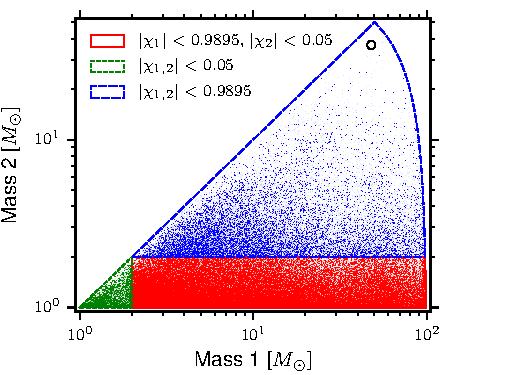
\includegraphics[width=\textwidth]{figs/chapter2/uberbank_boundaries.pdf}
\caption{The four-dimensional search parameter space covered by the template
bank shown projected into the component-mass plane, using the convention 
$m_1 > m_2$. The lines bound mass regions with different limits on the
dimensionless aligned-spin parameters $\chi_1$ and $\chi_2$. Each point
indicates the position of a template in the bank. The circle highlights the
template that best matches GW150914. This does not coincide with the best-fit
parameters due to the discrete nature of the template bank.
\label{fig:uberbank_boundaries}}
\end{figure}

For binary component objects with masses less than $2\,\Msun$, we limit the
magnitude of the component object's spin to $0.05$, the spin of the fastest
known pulsar in a double neutron star system~\cite{Burgay:2003jj}. At current
detector sensitivity, this is sufficient to detect gravitational-wave signals
from mergers of binaries with neutron star components having spins up to
$0.4$, the spin of the fastest-spinning millisecond
pulsar~\cite{Lorimer:2008se}.  Observations of X-ray binaries indicate that
astrophysical black holes may have near extremal
spins~\cite{McClintock:2013vwa}. For binary components with masses larger than
$2 \Msun$, we limit the spin magnitude to less than $0.9895$.  This is set by
our ability to generate valid template waveforms at higher
spins~\cite{Taracchini:2013rva}.  Figure~\ref{fig:uberbank_boundaries} shows the
boundaries of the search parameter space in the component-mass plane.
 

Since the parameters of signals are not known in advance, each detector's
output is filtered against a discrete bank of templates that span the search
target
space~\cite{Sathyaprakash:1991mt,Owen:1995tm,Owen:1998dk,Babak:2006ty,Cokelaer:2007kx}.
The placement of templates depends on the shape of the power spectrum of the
detector noise. Both analyses use a low-frequency cutoff of $30$~Hz for the search. 
The average noise power spectral density of the LIGO detectors
was measured over the period September 12 to September 26, 2015. The harmonic
mean of these noise spectra from the two detectors was used to place a single
template bank that was used for the duration of the
search~\cite{Keppel:2013uma,Usman:2015kfa}. The templates are placed using a combination of
geometric and stochastic
methods~\cite{Harry:2009ea,Brown:2012qf,Privitera:2013xza,Capano:2016uif}
such that the loss in matched-filter SNR caused by its discrete nature is
$\lesssim 3$\%.  Approximately 250,000 template waveforms are used to cover
this parameter space, as shown in Fig.~\ref{fig:uberbank_boundaries}.  The
performance of the template bank is tested numerically by simulating binary
black hole waveforms and determining the fraction of the total possible
matched-filter SNR recovered for each simulated signal (the fitting
factor)~\cite{Apostolatos:1996rf}.  Figure~\ref{fig:uberbank_effectualness}
shows the resulting distribution of fitting factors obtained over the
observation period. The loss in matched-filter SNR is less than $3\%$ for more
than $99$\% of the $10^5$ simulated signals.
\begin{figure}[t]
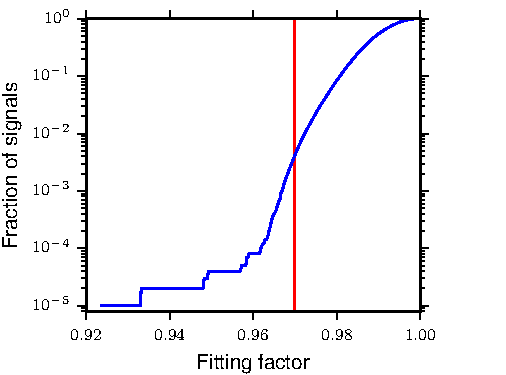
\includegraphics[width=\columnwidth]{figs/chapter2/uberbank_effectualness.pdf} 
\caption{\label{fig:uberbank_effectualness}
Cumulative distribution of fitting factors obtained with the template bank for
a  population of simulated aligned-spin binary black hole signals.  Less than $1\%$ of the
signals have an matched-filter SNR loss greater than $3\%$, demonstrating that the
template bank has good coverage of the target search space.}
\end{figure}

The template bank assumes that the spins of the two compact objects are
aligned with the orbital angular momentum. The resulting templates can
nonetheless effectively recover systems with misaligned spins in the
parameter-space region of GW150914. Figure~\ref{fig:precessing_effective_ff}
shows the effective fitting factor for simulated signals from a population of
simulated precessing binary black holes that are uniform in co-moving
volume~\cite{Pan:2013rra,HarryetalInPrep}. The effective fitting factor
weights the fraction of the matched-filter SNR recovered by the amplitude of
the signal~\cite{BuonannoChenVallisneri:2003b}. A signal that has a low
fitting factor may also have a poor orientation. When its strain is projected
onto the detector, the amplitude of the signal may be too small to detect even
if there was no mismatch between the signal and the template; the weighting in
the effective fitting accounts for this.  The effective fitting factor is
lowest at high mass ratios and low total mass, where the effects of precession
are more pronounced. In the region close to the parameters of GW150914  the
aligned-spin template bank is sensitive to a large fraction of precessing
signals~\cite{HarryetalInPrep}.
\begin{figure}[t]
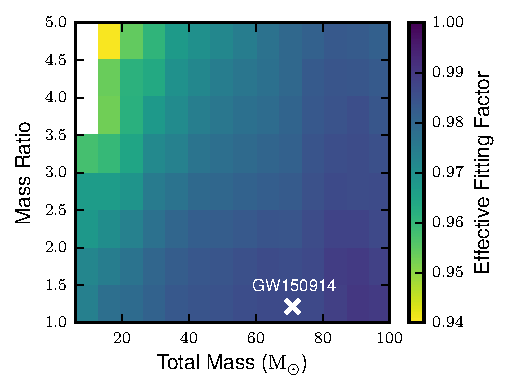
\includegraphics[width=\textwidth]{figs/chapter2/eff_ff_prec.pdf}
\caption{\label{fig:precessing_effective_ff}
The effective fitting factor between simulated precessing binary black hole
signals and the template bank used for the search as a function of
detector-frame total mass and mass ratio, averaged over each rectangular tile.
The effective fitting factor gives the volume-averaged reduction in the
sensitive distance of the search at fixed matched-filter SNR due to mismatch
between the template bank and signals.  The cross shows the location of
\TheEvent{}. The high effective fitting factor near GW150914 demonstrates that
the aligned-spin template bank used in this search can effectively recover
systems with misaligned spins and similar masses to GW150914.}
\end{figure}

In addition to possible gravitational-wave signals, the detector strain
contains a stationary noise background that primarily arises from photon shot
noise at high frequencies and seismic noise at low frequencies.  In the
mid-frequency range, detector commissioning has not yet reached the point
where test mass thermal noise dominates, and the noise at mid frequencies is
poorly
understood~\cite{GW150914-DETECTORS,GW150914-DETCHAR,InstrumentNoisePaper}.
The detector strain data also exhibits non-stationarity and non-Gaussian noise
transients that arise from a variety of instrumental or environmental
mechanisms. The measured strain $s(t)$ is the sum of possible
gravitational-wave signals $h(t)$ and the different types of detector noise
$n(t)$.

To monitor environmental disturbances and their influence on the detectors,
each observatory site is equipped with an array of
sensors~\cite{Effler:2014zpa}.  Auxiliary instrumental channels also record
the interferometer's operating point and the state of the detector's control
systems. Many noise transients have distinct signatures, visible in
environmental or auxiliary data channels that are not sensitive to
gravitational waves. When a noise source with known physical coupling between
these channels and the detector strain data is active, a data-quality veto is
created that is used to exclude these data from the
search~\cite{GW150914-DETCHAR}.
In the \pycbc{} analysis, these data quality vetoes are applied after filtering.  A
total of \CatTwoVetoTime{}~hours is removed from the analysis by data quality
vetoes.  Despite these detector characterization investigations, the data
still contains non-stationary and non-Gaussian noise which can affect the
astrophysical sensitivity of the search. Both analyses implement methods to
identify loud, short-duration noise transients and remove them from the strain
data before filtering.


The \pycbc{} analysis calculates the matched-filter SNR for each
template and each detector's data~\cite{Allen:2005fk,Cannon2010}.  In the
\pycbc{} analysis, sources with total mass less than 4$\,$\Msun~are modeled by
computing the inspiral waveform accurate to third-and-a-half post-Newtonian
order~\cite{Blanchet:1995ez,Droz:1999qx,Blanchet:2004ek}.  To model systems
with total mass larger than 4$\,$\Msun,~we use templates based on the
effective-one-body (EOB) formalism~\cite{Buonanno:2000ef}, which combines
results from the Post-Newtonian
approach~\cite{Blanchet:1995ez,Blanchet:2004ek} with results from black hole
perturbation theory and numerical
relativity~\cite{Taracchini:2013rva,Puerrer:2014fza} to model the complete
inspiral, merger and ringdown waveform.  The waveform models used assume that
the spins of the merging objects are aligned with the orbital angular
momentum. The analysiss then identifies maxima of the matched-filter SNR (triggers)
over the signal time of arrival.

To suppress large SNR values caused by non-Gaussian detector noise, the two
analyses calculate additional tests to quantify the agreement between the data
and the template.  The \pycbc{} analysis calculates a chi-squared statistic to
test whether the data in several different frequency bands are consistent with
the matching template~\cite{Allen:2004gu}.  The value of the chi-squared
statistic is used to compute a re-weighted SNR for each maxima.

The \pycbc{} analysis enforces coincidence between detectors by selecting trigger pairs
that occur within a $15\,$ms window and come from the same template.  The
$15\,$ms window is determined by the $10\,$ms inter-site propagation time plus
$5\,$ms for uncertainty in arrival time of weak signals.  The \pycbc{}
analyses discards any triggers that occur during the time of data-quality
vetoes prior to computing coincidence. The remaining coincident events are
ranked based on the quadrature sum of the re-weighted SNR from both
detectors~\cite{Usman:2015kfa}.

The significance of a candidate event is determined by the search background.
This is the rate at which detector noise produces events with a
detection-statistic value equal to or higher than the candidate event (the
false alarm rate).  Estimating this background is challenging for two reasons:
the detector noise is non-stationary and non-Gaussian, so its properties must
be empirically determined; and it is not possible to shield the detector from
gravitational waves to directly measure a signal-free background.  The
specific procedure used to estimate the background is different for the two
analyses.

To measure the significance of candidate events, the \pycbc{} analysis
artificially shifts the time\-stamps of one detector's triggers by an offset
that is large compared to the inter-site propagation time, and a new set of
coincident events is produced based on this time-shifted data set. For
instrumental noise that is uncorrelated between detectors this is an effective
way to estimate the background.  To account for the search background noise
varying across the target signal space, candidate and background events are
divided into three search classes based on template length. To account for
having searched multiple classes, the measured significance is decreased by a
trials factor equal to the number of classes~\cite{Lyons:1900zz}.  

The result of the independent analyses are two separate lists of candidate
events, with each candidate event assigned a p-value and false
alarm rate. These quantities are used to determine if a gravitational-wave
signal is present in the search.

\section{\pycbc{} Analysis}
\label{s:pycbc}

The \pycbc{} analysis~\cite{Canton:2014ena,Usman:2015kfa,pycbc-github}  uses
fundamentally the same
methods~\cite{Brown:2004pv,Allen:2005fk,Allen:2004gu,Brown:2005zs,Babak:2012zx,Brown:workflow,deelman2005pegasus,deelman2015pegasus,condor-practice,condor-dagman}
as those used to search for gravitational waves from compact binaries in the
initial LIGO and Virgo detector
era~\cite{Abbott:2003pj,Abbott:2005pe,Abbott:2005pf,Abbott:2005kq,Abbott:2007xi,Abbott:2007ai,Abbott:2009tt,Abbott:2009qj,Abadie:2010yba,Colaboration:2011np,Aasi:2012rja,Aasi:2014bqj},
with the improvements described in Refs.~\cite{Canton:2014ena,Usman:2015kfa}.
In this Section, we describe the configuration and tuning of the \pycbc{}
analysis used in this search.  To prevent bias in the search result, the
configuration of the analysis was determined using data taken prior to the
observation period searched. When GW150914 was discovered by the low-latency
transient searches~\cite{GW150914-DETECTION}, all tuning of the \pycbc{}
analysis was frozen to ensure that the reported p-values are
unbiased. No information from the low-latency transient search is used in this
analysis.

Of the \TotalCoincAfterCATOne~days of data that are used as input to the
analysis, the \pycbc{} analysis discards times for which either of the LIGO
detectors is in their observation state for less than $2064$\,s; shorter
intervals are considered to be unstable detector operation by this analysis
and are removed from the observation time. After discarding time removed by
data-quality vetoes and periods when detector operation is considered unstable
the observation time remaining is $\OBSDAYS$.

For each template $h(t)$ and for the strain data from a single detector
$s(t)$, the analysis calculates the square of the matched-filter SNR defined
by~\cite{Allen:2005fk}
\begin{equation}
  \label{eqn:matched_filter_snr}
  \rho^2(t) \equiv \frac{1}{\langle h | h \rangle} \left| \langle s | h \rangle(t) \right|^2,
\end{equation}
where the correlation is defined by 
\begin{equation}
 \langle s|h\rangle(t) = 4 \int^\infty_0 \frac{\tilde{s}(f)\tilde{h}^*(f)}{S_n(f)} e^{2\pi i ft}\,\dd f\,,
 \label{eqn:matched_filter_innerprod}
\end{equation}
where $\tilde{s}(f)$ is the Fourier transform of the time domain quantity $s(t)$
given by
\begin{equation}
\tilde{s}(f) = \int_{-\infty}^{\infty} s(t) e^{-2\pi ift}\,\dd t.
\end{equation}
The quantity $S_n(|f|)$ is the one-sided average power spectral density of the
detector noise, which is re-calculated every 2048\,s (in contrast to the fixed
spectrum used in template bank construction).  Calculation of the
matched-filter SNR in the frequency domain allows the use of the
computationally efficient Fast Fourier Transform~\cite{intel-mkl,FFTW05}.  The
square of the matched-filter SNR in Eq.~(\ref{eqn:matched_filter_snr}) is
normalized by
\begin{equation}
 \langle h|h\rangle = 4 \int^\infty_0 \frac{\tilde{h}(f)\tilde{h}^*(f)}{S_n(f)} \,\dd f\,,
 \label{eqn:matched_filter_norm}
\end{equation}
so that its mean value is $2$, if $s(t)$ contains only stationary
noise~\cite{Cutler:1994}.

Non-Gaussian noise transients in the detector can produce extended periods of
elevated matched-filter SNR that increase the search
background~\cite{Usman:2015kfa}. To mitigate this, a time-frequency excess
power (burst) search~\cite{Robinet:2015om} is used to identify high-amplitude,
short-duration transients that are not flagged by data-quality vetoes. If the
burst search generates a trigger with a burst SNR exceeding $300$, the
\pycbc{} analysis vetoes these data by zeroing out $0.5$s of $s(t)$ centered
on the time of the trigger. The data is smoothly rolled off using a Tukey
window during the $0.25$\,s before and after the vetoed data. The threshold of
$300$ is chosen to be significantly higher than the burst SNR obtained from
plausible binary signals. For comparison, the burst SNR of GW150914 in the
excess power search is $\sim 10$. A total of $450$ burst-transient vetoes are
produced in the two detectors, resulting in $225$\,s of data removed from the
search. A time-frequency spectrogram of the data at the time of each
burst-transient veto was inspected to ensure that none of these windows
contained the signature of an extremely loud binary coalescence.
\begin{figure}[t]
 \vspace*{-0.15in}
 \hspace*{-0.02\columnwidth}
 \subfloat[H1, 16 $\chi^2$ bins]{%
 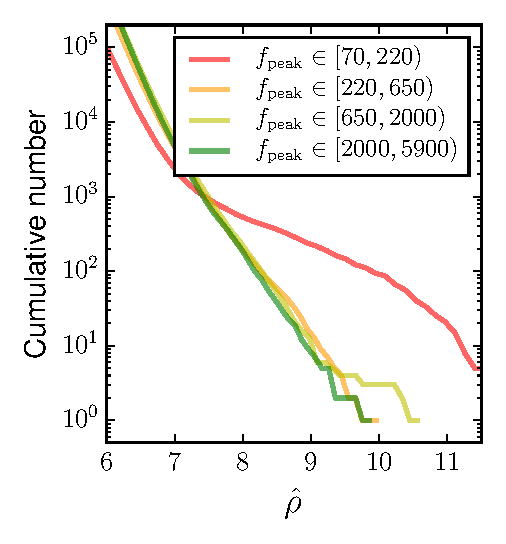
\includegraphics[height=0.45\textwidth]{figs/chapter2/H1-pycbc_sngl_trig_hists_before.pdf}%
 }
 \subfloat[H1, optimized $\chi^2$ bins]{%
 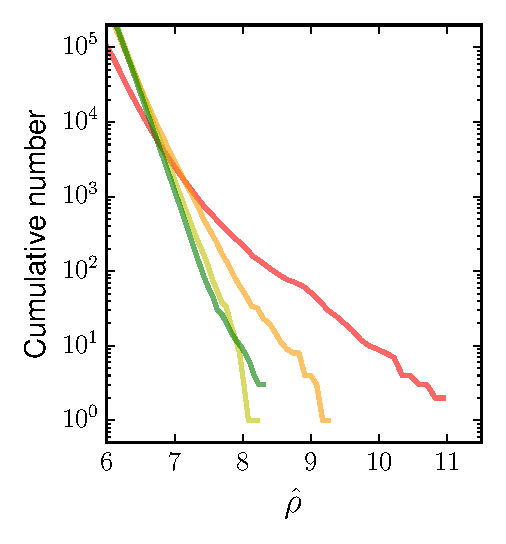
\includegraphics[trim={0.65in 0 0 0}, clip, height=0.45\textwidth]{figs/chapter2/H1-pycbc_sngl_trig_hists_after.pdf}%
 }
\\
 \hspace*{-0.02\columnwidth}
 \subfloat[L1, 16 $\chi^2$ bins]{%
 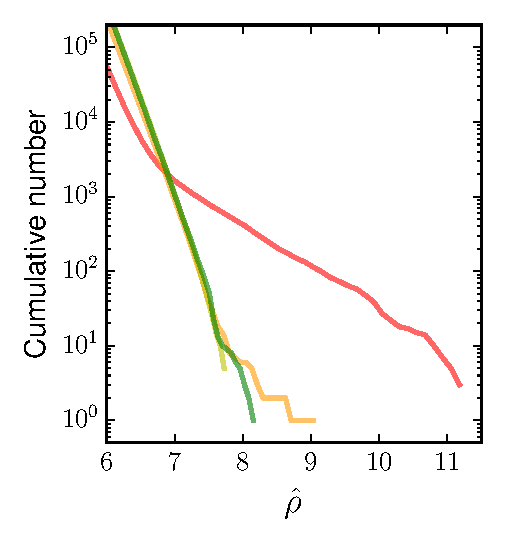
\includegraphics[height=0.45\textwidth]{figs/chapter2/L1-pycbc_sngl_trig_hists_before.pdf}%
 }
 \subfloat[L1, optimized $\chi^2$ bins]{%
 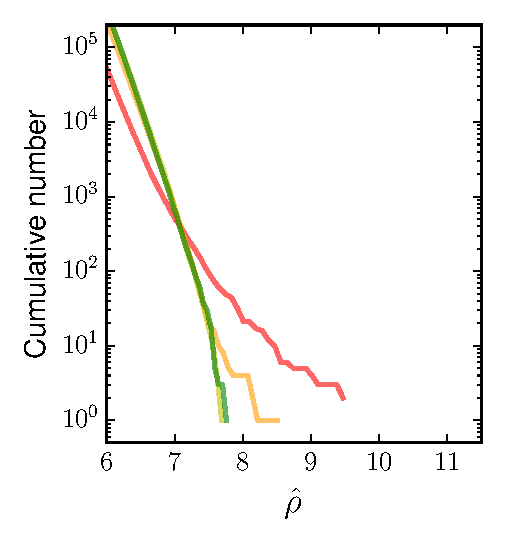
\includegraphics[trim={0.65in 0 0 0}, clip, height=0.45\textwidth]{figs/chapter2/L1-pycbc_sngl_trig_hists_after.pdf}%
 }
\caption{\label{fig:chisq_and_template_bins}
Distributions of noise triggers over re-weighted SNR $\hat{\rho}$, for
Advanced LIGO engineering run data taken between September 2 and September 9,
2015.  Each line shows triggers from templates within a given range of
gravitational-wave frequency at maximum strain amplitude, $f_\text{peak}$.
Left: Triggers obtained from H1, L1 data respectively, using a fixed number of
$p=16$ frequency bands for the $\chi^2$ test.  Right: Triggers obtained with
the number of frequency bands determined by the function $p=\lfloor 0.4
(f_\mathrm{peak}/\mathrm{Hz})^{2/3} \rfloor$.  Note that while noise
distributions are suppressed over the whole template bank with the optimized
choice of $p$, the suppression is strongest for templates with lower
$f_\mathrm{peak}$ values. Templates that have a $f_\text{peak} < 220\,$Hz
produce a large tail of noise triggers with high re-weighted SNR even with the
improved $\chi^2$-squared test tuning, thus we separate these templates from
the rest of the bank when calculating the noise background.
}
\end{figure}

The analysis places a threshold of $5.5$ on the single-detector matched-filter
SNR and identifies maxima of $\rho(t)$  with respect to the time of arrival of
the signal. For each maximum we calculate a chi-squared statistic to determine
whether the data in several different frequency bands are consistent with the
matching template~\cite{Allen:2004gu}. Given a specific number of frequency
bands $p$, the value of the reduced $\chi_r^2$ is given by
\begin{equation}
\chi_r^2 = \frac{p}{2p-2} \frac{1}{\langle h | h \rangle} \sum_{i=1}^p  \left|\langle s | h_i\rangle - \frac{\langle s | h\rangle}{p}\right|^2,
\label{eqn:pycbc_chisq}
\end{equation}
where $h_i$ is the sub-template corresponding to the $i$-th
frequency band.  Values of $\chi_r^2$ near unity indicate that the signal is
consistent with a coalescence. To suppress triggers from noise transients with
large matched-filter SNR, $\rho(t)$ is re-weighted
by~\cite{Colaboration:2011np,Babak:2012zx}
\begin{equation}
\hat{\rho} = \left\{\begin{array}{lr}
\rho\left/\left[(1+(\chi^2_r)^3)/2\right]^\frac{1}{6}\right., & \text{if } \chi_r^2 > 1, \\
\rho, & \text{if } \chi_r^2 \le 1.
\end{array}\right.
\end{equation}
Triggers that have a re-weighted SNR $\hat{\rho} < 5$ or that occur during
times subject to data-quality vetoes are discarded.

The template waveforms span a wide region of time-frequency parameter space
and the susceptibility of the analysis to a particular type of noise transient
can vary across the search space. This is demonstrated in
Fig.~\ref{fig:chisq_and_template_bins} which shows the cumulative number of
noise triggers as a function of re-weighted SNR for Advanced LIGO engineering
run data taken between September 2 and September 9, 2015. The response of the
template bank to noise transients is well characterized by the
gravitational-wave frequency at the template's peak amplitude,
$f_\mathrm{peak}$. Waveforms with a lower peak frequency have less cycles in
the detector's most sensitive frequency band from
$30$--$2000$\,Hz~\cite{GW150914-DETECTORS,InstrumentNoisePaper}, and so are
less easily distinguished from noise transients by the re-weighted SNR. 

The number of bins in the $\chi^2$ test is a tunable parameter in the
analysis~\cite{Usman:2015kfa}. Previous searches used a fixed number of
bins~\cite{Babak:2005kv} with the most recent Initial LIGO and Virgo searches
using $p=16$ bins for all templates~\cite{Colaboration:2011np,Aasi:2012rja}.
Investigations on data from LIGO's sixth science
run~\cite{AlexNitzThesis,Aasi:2012rja} showed that better noise rejection is
achieved with a template-dependent number of bins.  The left two panels of
Fig.~\ref{fig:chisq_and_template_bins} show the cumulative number of noise
triggers with $p = 16$ bins used in the $\chi^2$ test.  Empirically, we find
that choosing the number of bins according to
\begin{equation}
p=\lfloor 0.4 (f_\mathrm{peak}/\mathrm{Hz})^{2/3}\rfloor
\label{eq:chisq_bins}
\end{equation}
gives better suppression of noise transients in Advanced LIGO data, as shown
in the right panels of Fig.~\ref{fig:chisq_and_template_bins}.

The \pycbc{} analysis enforces signal coincidence between detectors by
selecting trigger pairs that occur within a $15\,$ms window and come from the
same template.   We rank coincident events based on the quadrature sum
$\hat{\rho}_c$ of the $\hat{\rho}$ from both detectors~\cite{Usman:2015kfa}.
The final step of the analysis is to cluster the coincident events, by
selecting those with the largest value of $\hat{\rho}_c$ in each time window
of $10$\,s. Any other events in the same time window are discarded.  This
ensures that a loud signal or transient noise artifact gives rise to at most
one candidate event~\cite{Usman:2015kfa}. 

The significance of a candidate event is determined by the rate at which
detector noise produces events with a detection-statistic value equal to or
higher than that of the candidate event. To measure this, the analysis creates
a ``background data set" by artificially shifting the time\-stamps of one
detector's triggers by many multiples of $0.1$\,s and computing a new set of
coincident events.  Since the time offset used is always larger than the
time-coincidence window, coincident signals do not contribute to this
background. Under the assumption that noise is not correlated between the
detectors~\cite{GW150914-DETCHAR}, this method provides an unbiased estimate
of the noise background of the analysis. 

To account for the noise background varying across the target signal space,
candidate and background events are divided into different search classes
based on template length.  Based on empirical tuning using Advanced LIGO
engineering run data taken between September 2 and September 9, 2015, we
divide the template space into three classes according to: (i) $\mathcal{M} <
1.74\,\Msun$; (ii) $\mathcal{M}
\geq 1.74\,\Msun$ and $f_\mathrm{peak} \geq 220\,$Hz; (iii) $\mathcal{M} \geq 1.74\,\Msun$
and $f_\mathrm{peak} < 220\,$Hz.  The significance of candidate events is
measured against the background from the same class.  For each candidate
event, we compute the \fap{}. This is the probability
of finding one or more noise background events in the observation time with a
detection-statistic value above that of the candidate event, given
by~\cite{Usman:2015kfa, Capano:2016uif}
\begin{equation} 
\begin{split}
\label{eq:pycbc_slide_fap}
 \fap(\hat{\rho}_c) \equiv P(\geq 1\;\text{noise event above}\;\hat{\rho}_c|T, T_b) = \\
 1 - \exp\left[ -T \frac{1+n_b(\hat{\rho}_c)}{T_b} \right],
\end{split}
\end{equation}
where $T$ is the observation time of the search, $T_b$ is the background time,
and $n_b(\hat{\rho}_c)$ is the number of noise background triggers above the
candidate event's re-weighted SNR $\hat{\rho}_c$. 

Eq.~(\ref{eq:pycbc_slide_fap}) is derived assuming Poisson statistics for the
counts of time-shifted background events, and for the count of coincident
noise events in the search~\cite{Usman:2015kfa, Capano:2016uif}.  This
assumption requires that different time-shifted analyses (i.e.\ with different
relative shifts between detectors) give independent realizations of a counting
experiment for noise background events. We expect different time shifts to
yield independent event counts since the $0.1$\,s offset time is greater than
the $10$\,ms gravitational-wave travel time between the sites plus the $\sim
1$\,ms autocorrelation length of the templates. To test the independence of
event counts over different time shifts over this observation period, we
compute the differences in the number of background events having $\rwRhoC >
9$ between consecutive time shifts.  Figure~\ref{fig:slide_corr} shows that the
measured differences on these data follow the expected distribution for the
difference between two independent Poisson random
variables~\cite{Skellam:1946}, confirming the independence of time shifted
event counts. 
\begin{figure}[!t]
\hspace*{-0.1in}
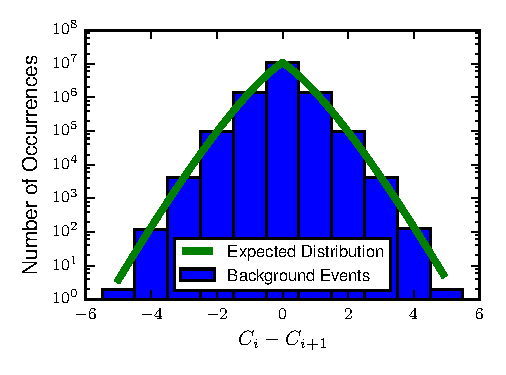
\includegraphics[width=\textwidth]{figs/chapter2/slide_corr.pdf}
\caption{\label{fig:slide_corr} 
The distribution of the differences in the number of events between 
consecutive time shifts, where $C_i$ denotes the number of events in the 
$i$th time shift.
The green line shows the predicted distribution for independent Poisson
processes with means equal to the average event rate per time shift. 
The blue histogram shows the distribution obtained from time-shifted 
analyses.  The variance of the time-shifted background distribution is 
1.996, consistent with the predicted variance of 2. The distribution 
of background event counts in adjacent time shifts is well modeled by 
independent Poisson processes.}
\end{figure}

If a candidate event's detection-statistic value is larger than that of any
noise background event, as is the case for GW150914, then the \pycbc{}
analysis places an upper bound on the candidate's $p$-value.
After discarding time removed by data-quality vetoes and periods when the
detector is in stable operation for less than $2064$~seconds, the total
observation time remaining is $T= \OBSDAYS$.  Repeating the time-shift
procedure {\PYCBCHOWMANYTIMESLIDES} times on these data produces a noise
background analysis time equivalent to $T_b=\PYCBCBCKLIVETIME$ years.  Thus,
the smallest $p$-value that can be estimated in this analysis is
approximately $7\times 10^{-8}$. Since we treat the search parameter
space as \PYCBCTRIALFACTOR{} independent classes, each of which may generate a
false positive result, this value should be multiplied by a trials factor or
look-elsewhere effect~\cite{Lyons:1900zz} of \PYCBCTRIALFACTOR{}, resulting in
a minimum measurable $\fap = 2\times 10^{-7}$.  The
results of the \pycbc{} analysis are described in Sec.~\ref{s:results}.

\section{Search Results}
\label{s:results}

GW150914 was observed on \OBSEVENTDATEMONTHDAYYEAR\ at \OBSEVENTTIME
~\OBSEVENTTZ\ as the most significant event by both analyses. The individual
detector triggers from GW150914 occurred within the 10\,ms inter-site
propagation time with a combined matched-filter SNR of
\OBSEVENTAPPROXCOMBINEDSNR. Both pipelines report the same matched-filter SNR
for the individual detector triggers in the Hanford detector
($\rho_\textrm{H1} = 20$) and the Livingston detector ($\rho_\textrm{L1} =
13$).  GW150914 was found with the same template in both analyses with
component masses $\CBCEventTemplateMassOne\,\Msun$ and
$\CBCEventTemplateMassTwo\,\Msun$. The effective spin of the best-matching
template is $\chi_{\text{eff}} = (c/G) (\mathbf{S_1}/m_1 + \mathbf{S_2}/m_2)
\cdot (\mathbf{\hat{L}}/M) = 0.2$, where $\mathbf{S_{1,2}}$ are the spins of
the compact objects and $\mathbf{\hat{L}}$ is the direction of the binary's
orbital angular momentum. Due to the discrete nature of the template bank,
follow-up parameter estimation is required to accurately determine the best
fit masses and spins of the binary's components~\cite{Veitch:2014wba,
GW150914-PARAMESTIM}. 

The frequency at peak amplitude of the best-matching template is
$f_{\mathrm{peak}} = \CBCEventPeakFrequency\,$Hz, placing it in
noise-background class (iii) of the \pycbc{} analysis.
Figure~\ref{fig:both_results} (left) shows the result of the \pycbc{} analysis
for this search class.  In the time-shift analysis used to create the noise
background estimate for the \pycbc{} analysis, a signal may contribute events
to the background through random coincidences of the signal in one
detector with noise in the other detector~\cite{Capano:2016uif}.  This can be
seen in the background histogram shown by the black line. The tail is due
to coincidence between the single-detector triggers from GW150914 and noise in
the other detector.  If a loud signal is in fact present, these random
time-shifted coincidences contribute to an overestimate of the noise
background and a more conservative assessment of the significance of an event.
Figure~\ref{fig:both_results} shows that GW150914 has a re-weighted SNR
$\rwRhoC = \PycbcEventNewSNR$, greater than all background events in its
class. This value is also greater than all background in the other two
classes. As a result, we can only place an upper bound on the false alarm
rate, as described in Sec.~\ref{s:pycbc}. This bound is equal to the number of
classes divided by the background time $T_b$. With $3$ classes and $T_b =
\PYCBCBCKLIVETIME$ years, we find the false alarm rate of GW150914 to be less
than $\CBCEVENTFAR\,\text{yr}^{-1}$. With an observing time of $\OBSHOURS$,
the $\fap~\CBCEVENTFAPBOUND$.  Converting this
$p$-value to single-sided Gaussian standard deviations according
to $-\sqrt{2}\ \mathrm{erf}^{-1}\left[1 - 2(1-\fap)\right]$, where
$\mathrm{erf}^{-1}$ is the inverse error function, the \pycbc{} analysis
measures the significance of GW150914 as greater than \CBCEVENTSIGMA
$\,\sigma$. 
\begin{figure*}[t!]
\centering
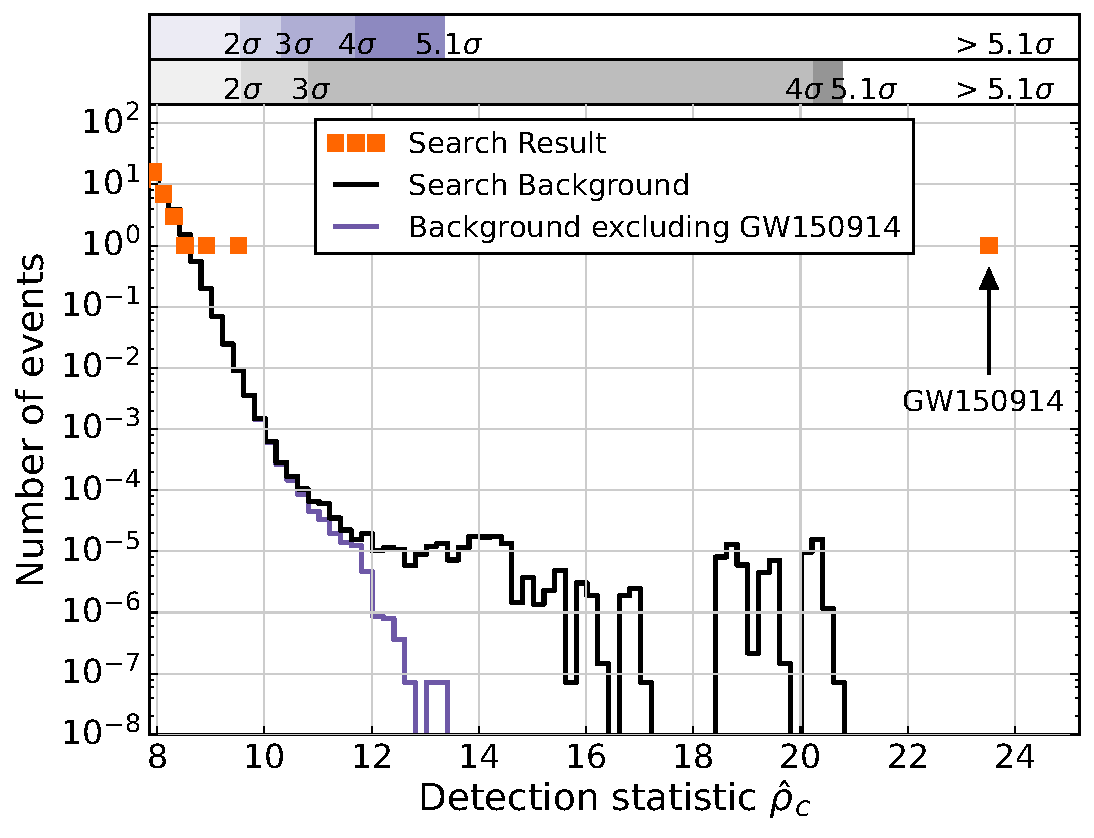
\includegraphics[width=\textwidth]{figs/chapter2/pycbc-hist-0p1s-sigmas.pdf}
\caption{Left: Search results from the \pycbc{} analysis. The histogram shows
the number of candidate events (orange) and the number of background events
due to noise in the search class where GW150914 was found (black) as a
function of the search detection-statistic and with a bin width of $\Delta
\hat{\rho}_c = 0.2$. The significance of GW150914 is greater than
{\CBCEVENTSIGMA} $\sigma$.  The scales immediately above the histogram give
the significance of an event measured against the noise backgrounds in units
of Gaussian standard deviations as a function of the detection-statistic.  The
black background histogram shows the result of the time-shift method to
estimate the noise background in the observation period. The tail in the
black-line background of the binary coalescence search is due to random
coincidences of GW150914 in one detector with noise in the other detector. The
significance of GW150914 is measured against the upper gray scale.  The purple
background histogram is the background excluding coincidences involving
GW150914 and it is the background to be used to assess the significance of the
second loudest event; the significance of this event is measured against the
upper purple scale.}
\label{fig:both_results}
\end{figure*}

\begin{figure*}[t]
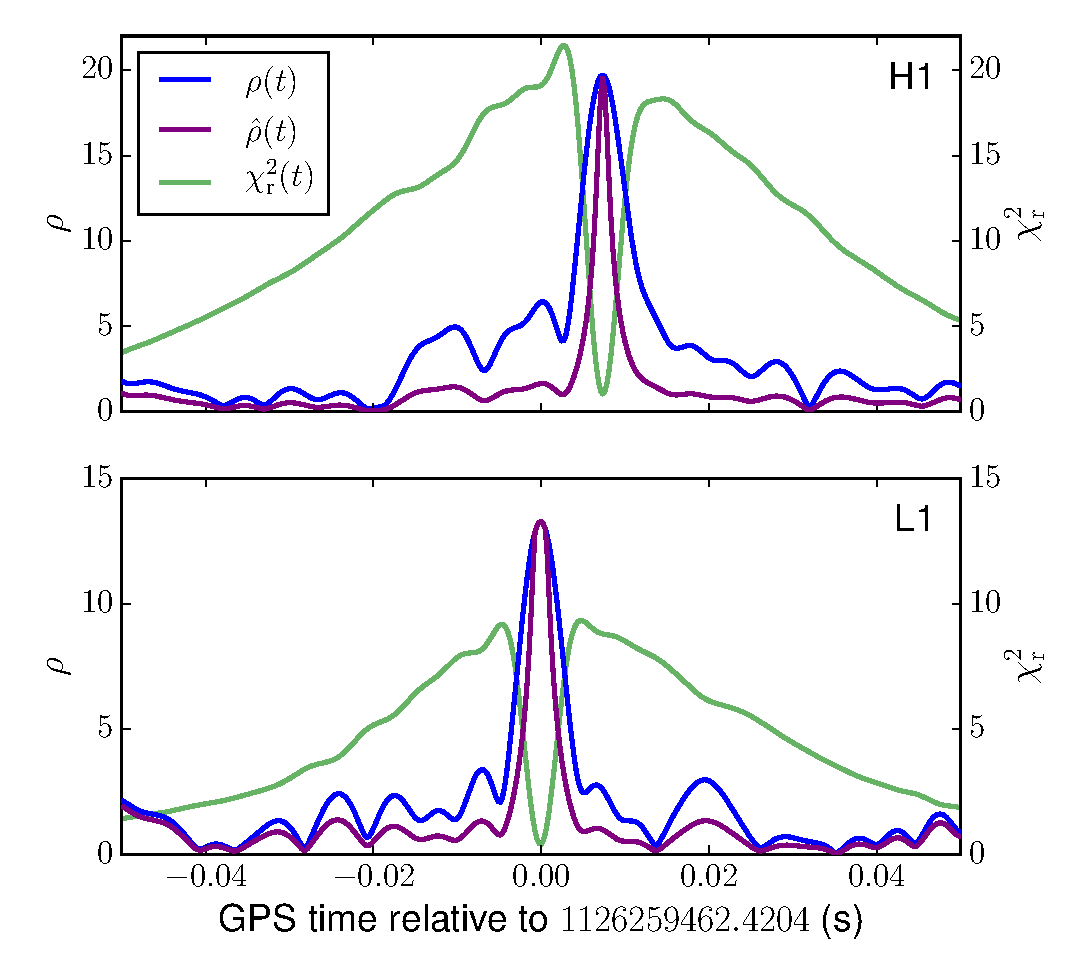
\includegraphics[width=\textwidth]{figs/chapter2/combined_single.pdf}
\caption{\label{fig:pycbc_gstlal_snr_chisq_vs_time}
PyCBC matched-filter SNR (blue), re-weighted SNR (purple) and $\chi^2$
(green) versus time of the best-matching template at the time of \TheEvent.
The top plot shows the Hanford detector; bottom, Livingston.
}
\end{figure*}

The difference in time of arrival between the Livingston and Hanford detectors
from the individual triggers in the \pycbc{} analysis is
$\CBCEventTimeDiff\,$ms, consistent with the time delay of
\TIMEDELAYCOMPACT\,ms recovered by parameter
estimation~\cite{GW150914-PARAMESTIM}.
Figure~\ref{fig:pycbc_gstlal_snr_chisq_vs_time} shows the
matched-filter SNR $\rho$, the $\chi^2$-statistic, and the re-weighted SNR
$\hat\rho$ for the best-matching template over a period of $\pm5$\,ms around
the time of GW150914 (we take the \pycbc{} trigger time in L1 as a reference).
The matched-filter SNR peaks in both detectors at the time of the event and
the value of the reduced chi-squared statistic is $\chi^2_\mathrm{H1} = 1$ and
$\chi^2_\mathrm{L1} = 0.7$ at the time of the event, indicating an excellent
match between the template and the data. The re-weighted SNR of the individual
detector triggers of $\hat{\rho}_\mathrm{H1} = 19.5$ and
$\hat{\rho}_\mathrm{L1} = 13.3$ are larger than that of any other
single-detector triggers in the analysis; therefore the significance
measurement of \CBCEVENTSIGMA $\,\sigma$ set using the $0.1$~s time shifts is
a conservative bound on the $p$-value of \TheEvent.

The \pycbc{} analysis has shown that the probability that GW150914 was formed by
random coincidence of detector noise is extremely small. We therefore conclude
that GW150914 is a gravitational-wave signal. To measure the signal
parameters, we use parameter estimation methods that assume the presence of a
coherent coalescing binary signal in the data from both
detectors~\cite{Veitch:2014wba,GW150914-PARAMESTIM}. Two waveform models were
used which included inspiral, merger and ring-down portions of the signal: one
which includes spin components aligned with orbital angular
momentum~\cite{Pan:2009wj,Puerrer:2014fza} and one which includes the dominant
modulation of the signal due to orbital precession caused by mis-aligned
spins~\cite{Hannam:2013oca,Khan:2015jqa}.  The parameter estimates are
described by a continuous probability density function over the source
parameters. We conclude that \TheEvent{} is a nearly equal mass black-hole
binary system of source-frame masses {\MONESCOMPACT~\Msun} and
{\MTWOSCOMPACT~\Msun} (median and $90\%$ credible range). The spin magnitude
of the primary black hole is constrained to be less than ${\SPINONELIMIT}$
with $90\%$ probability.  The most stringent constraint on the spins of the
two black holes is on the effective spin parameter $\chi_\mathrm{eff} =
\CHIEFFCOMPACT$.  The parameters of the best-fit template are consistent with
these values, given the discrete nature of the template bank.  We estimate
\TheEvent{} to be at a luminosity distance of
{\DISTANCECOMPACT~$\mathrm{Mpc}$}, which corresponds to a redshift
{\REDSHIFTCOMPACT}.  Full details of the source parameters for GW150914 are
given in Ref.~\cite{GW150914-PARAMESTIM} and summarized in
Table~\ref{tab:results}.

When an event is confidently identified as a real gravitational wave signal,
as for GW150914, the background used to determine the significance of other
events is re-estimated without the contribution of this event. This is the
background distribution shown as purple lines in Fig.~\ref{fig:both_results}.
Both analyses reported a candidate event on \SecondTime{} as the
second-loudest event in the observation period, which we refer to as
\SECONDMONDAY. This candidate event has a combined matched-filter SNR of
\PyCBCSecondEventRhoC.  The \pycbc{} analysis reported a false alarm rate of 1
per \CBCSECONDEVENTIFAR~years and a corresponding $p$-value of
\CBCSECONDEVENTFAP{} for this event.
Detector characterization studies have not identified an
instrumental or environmental artifact as causing this candidate event
\cite{GW150914-DETCHAR}, however its p-value is not
sufficiently low to confidently claim the event as a signal.  It is
significant enough to warrant follow-up, however.  The results of signal
parameter estimation, shown in Table~\ref{tab:results}, indicate that if
\SECONDMONDAY{} is of astrophysical origin, then the source would be a
stellar-mass binary black hole system with source-frame component masses
$\MONESCOMPACTSecondMonday\,\Msun$ and $\MTWOSCOMPACTSecondMonday\,\Msun$. The
effective spin would be $\chi_\mathrm{eff} = \CHIEFFCOMPACTSecondMonday$ and
the distance \DISTANCECOMPACTSecondMonday~Mpc.

\newpage

\begin{table*}[t]
\begin{adjustbox}{angle=90}
  \centering
  \begin{tabular}{c|c|c|c|c|c|c|c|c}
    Event & Time (UTC) & FAR (yr$^{-1}$) & $p$-value & $\mathcal{M}$ $(\Msun)$ & $m_1$ $(\Msun)$ & $m_2$ $(\Msun)$ & $\chi_{\mathrm{eff}}$ & $D_L$ (Mpc) \\
    \hline \hline
    \TheEvent{} & \CBCEventUTCTimeShort & $< \CBCEVENTFAR$ & $\CBCEVENTFAPBOUND$\newline$(> \CBCEVENTSIGMA\,\sigma)$ & \MCSCOMPACT & \MONESCOMPACT & \MTWOSCOMPACT &  \CHIEFFCOMPACT & \DISTANCECOMPACT \\
    \SECONDMONDAY{} & \CBCSecondEventUTCTimeShort & \CBCSECONDEVENTFAR & $\CBCSECONDEVENTFAP$\newline$(\PyCBCSecondEventSigma\,\sigma)$ &  \MCSCOMPACTSecondMonday & \MONESCOMPACTSecondMonday  & \MTWOSCOMPACTSecondMonday & \CHIEFFCOMPACTSecondMonday & \DISTANCECOMPACTSecondMonday \\
  \end{tabular}
\caption{\label{tab:results}  Parameters of the two most significant events. The false alarm rate (FAR) and
$p$-value given here were determined by the \pycbc{}
pipeline. The source-frame
chirp mass $\mathcal{M}$, component masses $m_{1,2}$, effective spin
$\chi_{\mathrm{eff}}$, and luminosity distance $D_L$ are determined using a
parameter estimation method that assumes the presence of a coherent compact
binary coalescence signal starting at 20\,Hz in the
data~\cite{Veitch:2014wba}. The results are computed by averaging the
posteriors for two model waveforms.  Quoted uncertainties are $90\%$ credible
intervals that include statistical errors and systematic errors from
averaging the results of different waveform models.  Further parameter
estimates of \TheEvent{} are presented in Ref.~\cite{GW150914-PARAMESTIM}.
In the chapter ~\ref{ch:1_OGC} we will investigate how improvements to
the \pycbc{} pipeline can improve the statistical significance estimate
of LVT151012.}
\end{adjustbox}
\end{table*}
